%%%%%%%%%%%%%%%%%%%%%%%%%%%%%%%%%%%%%%%%
% datoteka magistrska_naloga.tex
%
% vzorčna datoteka za pisanje magistrskega dela v formatu LaTeX
% na UL Fakulteti za računalništvo in informatiko
%
% pripravili: Zoran Bosnić, Andrej Čopar, po predlogi Gašperja Fijavža
% popravil: Matej Kristan
% verzija 10. september 2014

\documentclass[a4paper, 12pt]{book}

\usepackage[utf8]{inputenc}   % omogoča uporabo slovenskih črk kodiranih v formatu UTF-8
\usepackage[slovene,english]{babel}    % naloži, med drugim, slovenske delilne vzorce
\usepackage[style=ieee, backend=bibtex, language=slovene]{biblatex} % slovenski izpis referenc v IEEE
\usepackage[pdftex]{graphicx}  % omogoča vlaganje slik različnih formatov
\usepackage{fancyhdr}          % poskrbi, na primer, za glave strani
\usepackage{amssymb}           % dodatni simboli
\usepackage{amsmath}           % eqref, npr.
\usepackage{url}

%%%%%%%%%%%%%%%%%%%%%%%%%%%%%%%%%%%%%%%%
% prilagoditev robov za tisk
%%%%%%%%%%%%%%%%%%%%%%%%%%%%%%%%%%%%%%%%
\addtolength{\marginparwidth}{-20pt}
\addtolength{\oddsidemargin}{40pt}
\addtolength{\evensidemargin}{-40pt}

%%%%%%%%%%%%%%%%%%%%%%%%%%%%%%%%%%%%%%%%
% postavitev strani
%%%%%%%%%%%%%%%%%%%%%%%%%%%%%%%%%%%%%%%%
\renewcommand{\baselinestretch}{1.3} % ustrezen razmik med vrsticami

%oznake strani
\renewcommand{\chaptermark}[1]%
{\markboth{\MakeUppercase{\thechapter.\ #1}}{}} \renewcommand{\sectionmark}[1]%
{\markright{\MakeUppercase{\thesection.\ #1}}} \renewcommand{\headrulewidth}{0.5pt} \renewcommand{\footrulewidth}{0pt}
\fancyhf{}
\fancyhead[LE,RO]{\sl \thepage} \fancyhead[LO]{\sl \rightmark} \fancyhead[RE]{\sl \leftmark}

\newcommand{\BibTeX}{{\sc Bib}\TeX}

\newcommand{\autfont}{\Large}
\newcommand{\titfont}{\LARGE\bf}
\newcommand{\clearemptydoublepage}{\newpage{\pagestyle{empty}\cleardoublepage}}
\setcounter{tocdepth}{1}	      % globina kazala

%%%%%%%%%%%%%%%%%%%%%%%%%%%%%%%%%%%%%%%%
% konstrukti
%%%%%%%%%%%%%%%%%%%%%%%%%%%%%%%%%%%%%%%%
\newtheorem{izrek}{Izrek}[chapter]
\newtheorem{trditev}{Trditev}[izrek]
\newenvironment{dokaz}{\emph{Dokaz.}\ }{\hspace{\fill}{$\Box$}}

%%%%%%%%%%%%%%%%%%%%%%%%%%%%%%%%%%%%%%%%
%	INFO O MAGISTRSKI NALOGI: ustrezno zamenjaj
%%%%%%%%%%%%%%%%%%%%%%%%%%%%%%%%%%%%%%%%
\newcommand{\ttitle}{Interaktivne računalniške umetniške instalacije v času hitrega tehnološkega razvoja}
\newcommand{\ttitleEn}{Interactive computer-based art installations in times of rapid technological advances}
\newcommand{\tsubject}{\ttitle}
\newcommand{\tsubjectEn}{\ttitleEn}
\newcommand{\tauthor}{Gregor Majcen}
\newcommand{\tmentor}{prof.\ dr. Franc Solina}
\newcommand{\tkeywords}{računalnik, računalnik, računalnik}
\newcommand{\tkeywordsEn}{computer, computer, computer}



\usepackage{hyperref}
%%%%%%%%%%%%%%%%%%%%%%%%%%%%%%%%%%%%%%%%
%	HYPERREF SETUP: ustrezno popravi e-mail
%%%%%%%%%%%%%%%%%%%%%%%%%%%%%%%%%%%%%%%%
\hypersetup{pdftitle={\ttitle}}
\hypersetup{pdfsubject=\ttitleEn}
\hypersetup{pdfauthor={\tauthor}}
\hypersetup{pdfkeywords=\tkeywordsEn}


%%%%%%%%%%%%%%%%%%%%%%%%%%%%%%%%%%%%%%%%%%%%%%%%%%%%%%%%%%%%%%%%%%%%%%%%%%%%%%%
%% PDF-A
%%%%%%%%%%%%%%%%%%%%%%%%%%%%%%%%%%%%%%%%%%%%%%%%%%%%%%%%%%%%%%%%%%%%%%%%%%%%%%%

%%%%%%%%%%%%%%%%%%%%%%%%%%%%%%%%%%%%%%%%
% define medatata: ustrezno popravi e-mail
%%%%%%%%%%%%%%%%%%%%%%%%%%%%%%%%%%%%%%%%
\def\Title{\ttitle}
\def\Author{\tauthor}
\def\Subject{\ttitleEn}
\def\Keywords{\tkeywordsEn}

%%%%%%%%%%%%%%%%%%%%%%%%%%%%%%%%%%%%%%%%
% \convertDate converts D:20080419103507+02'00' to 2008-04-19T10:35:07+02:00
%%%%%%%%%%%%%%%%%%%%%%%%%%%%%%%%%%%%%%%%
\def\convertDate{%
    \getYear
}

{\catcode`\D=12
 \gdef\getYear D:#1#2#3#4{\edef\xYear{#1#2#3#4}\getMonth}
}
\def\getMonth#1#2{\edef\xMonth{#1#2}\getDay}
\def\getDay#1#2{\edef\xDay{#1#2}\getHour}
\def\getHour#1#2{\edef\xHour{#1#2}\getMin}
\def\getMin#1#2{\edef\xMin{#1#2}\getSec}
\def\getSec#1#2{\edef\xSec{#1#2}\getTZh}
\def\getTZh +#1#2{\edef\xTZh{#1#2}\getTZm}
\def\getTZm '#1#2'{%
    \edef\xTZm{#1#2}%
    \edef\convDate{\xYear-\xMonth-\xDay T\xHour:\xMin:\xSec+\xTZh:\xTZm}%
}

\expandafter\convertDate\pdfcreationdate

%%%%%%%%%%%%%%%%%%%%%%%%%%%%%%%%%%%%%%%%
% get pdftex version string
%%%%%%%%%%%%%%%%%%%%%%%%%%%%%%%%%%%%%%%%
\newcount\countA
\countA=\pdftexversion
\advance \countA by -100
\def\pdftexVersionStr{pdfTeX-1.\the\countA.\pdftexrevision}


%%%%%%%%%%%%%%%%%%%%%%%%%%%%%%%%%%%%%%%%
% XMP data
%%%%%%%%%%%%%%%%%%%%%%%%%%%%%%%%%%%%%%%%
\usepackage{xmpincl}
%\includexmp{styles/pdfa-1b}

%%%%%%%%%%%%%%%%%%%%%%%%%%%%%%%%%%%%%%%%
% pdfInfo
%%%%%%%%%%%%%%%%%%%%%%%%%%%%%%%%%%%%%%%%
\pdfinfo{%
    /Title    (\ttitle)
    /Author   (\tauthor)
    /Subject  (\ttitleEn)
    /Keywords (\tkeywordsEn)
    /ModDate  (\pdfcreationdate)
    /Trapped  /False
}

\graphicspath{{./figures/}}
\addbibresource{literatura}

%%%%%%%%%%%%%%%%%%%%%%%%%%%%%%%%%%%%%%%%%%%%%%%%%%%%%%%%%%%%%%%%%%%%%%%%%%%%%%%
%%%%%%%%%%%%%%%%%%%%%%%%%%%%%%%%%%%%%%%%%%%%%%%%%%%%%%%%%%%%%%%%%%%%%%%%%%%%%%%


\begin{document}
\selectlanguage{slovene}
\frontmatter
\setcounter{page}{1} %
\renewcommand{\thepage}{}       % preprecimo težave s številkami strani v kazalu

%%%%%%%%%%%%%%%%%%%%%%%%%%%%%%%%%%%%%%%%
%naslovnica
 \thispagestyle{empty}%
   \begin{center}
    {\large\sc Univerza v Ljubljani\\%
      Fakulteta za računalništvo in informatiko}%
    \vskip 10em%
    {\autfont \tauthor \par}%
    {\titfont \ttitle \par}%
    {\vskip 2em \textsc{MAGISTRSKO DELO\\[2mm]
    ŠTUDIJSKI PROGRAM DRUGE STOPNJE\\ RAČUNALNIŠTVO IN INFORMATIKA}\par}%
    \vfill\null%
    {\large \textsc{Mentor}: \tmentor \par}%
    {\vskip 2em \large Ljubljana, 2015 \par}%
\end{center}
% prazna stran
\clearemptydoublepage

%%%%%%%%%%%%%%%%%%%%%%%%%%%%%%%%%%%%%%%%
%copyright stran
\thispagestyle{empty}
\vspace*{8cm}
{\small \noindent
Rezultati magistrskega dela so intelektualna lastnina avtorja in Fakultete za ra\-ču\-nal\-niš\-tvo in informatiko Univerze v Ljubljani.
Za objavljanje ali izkoriščanje rezultatov ma\-gi\-str\-ske\-ga dela je potrebno pisno soglasje avtorja, Fakultete za ra\-ču\-nal\-niš\-tvo in
informatiko ter mentorja}



% prazna stran
\clearemptydoublepage

%%%%%%%%%%%%%%%%%%%%%%%%%%%%%%%%%%%%%%%%


%%%%%%%%%%%%%%%%%%%%%%%%%%%%%%%%%%%%%%%%
% izjava o avtorstvu
\vspace*{1cm}
\begin{center}
{\Large \textbf{\sc Izjava o avtorstvu magistrskega dela}}
\end{center}

\vspace{1cm}
\noindent Spodaj podpisani \tauthor{} sem avtor magistrskega dela z naslovom:

\vspace{0.5cm}
\emph{\ttitle}

\vspace{1.5cm}
\noindent S svojim podpisom zagotavljam, da:
\begin{itemize}
	\item sem magistrsko delo izdelal samostojno pod mentorstvom
		\tmentor,

	\item so elektronska oblika magistrskega dela, naslov (slov., angl.), povzetek (slov., angl.) ter ključne besede (slov., angl.) identični s tiskano obliko magistrskega dela,
	\item soglašam z javno objavo elektronske oblike magistrskega dela v zbirki ''Dela FRI''.
\end{itemize}

\vspace{1cm}
\noindent V Ljubljani, 11. marca 2014 \hfill Podpis avtorja:

% prazna stran
\clearemptydoublepage

%%%%%%%%%%%%%%%%%%%%%%%%%%%%%%%%%%%%%%%%
% zahvala
\thispagestyle{empty}\mbox{}\vfill\null\it%
Na tem mestu zapišite, komu se zahvaljujete za izdelavo magistrske naloge. V zahvali se poleg mentorja spodobi omeniti vse, ki so s svojo pomočjo prispevali k nastanku vašega izdelka.

\rm\normalfont

% prazna stran
\clearemptydoublepage

%%%%%%%%%%%%%%%%%%%%%%%%%%%%%%%%%%%%%%%%
% posvetilo
\thispagestyle{empty}\mbox{}{\vskip0.20\textheight}\mbox{}\hfill\begin{minipage}{0.55\textwidth}%
Tebi, ki si moje sonce, ki prežene oblake.\\
{\it (morebitno posvetilo)}
\normalfont\end{minipage}

% prazna stran
\clearemptydoublepage

%%%%%%%%%%%%%%%%%%%%%%%%%%%%%%%%%%%%%%%%
% kazalo
\def\thepage{}% preprecimo tezave s stevilkami strani v kazalu
\tableofcontents{}


% prazna stran
\clearemptydoublepage

%%%%%%%%%%%%%%%%%%%%%%%%%%%%%%%%%%%%%%%%
% seznam kratic

\chapter*{Seznam uporabljenih kratic}

\begin{tabular}{l|l|l}
  {\bf kratica} & {\bf angleško} & {\bf slovensko} \\ \hline
  % after \\: \hline or \cline{col1-col2} \cline{col3-col4} ...
  {\bf CA} & classification accuracy & klasifikacijska točnost \\
  {\bf DBMS} & database management system & sistem za upravljanje podatkovnih baz \\
  {\bf SVM} & support vector machine & metoda podpornih vektorjev \\
  ... & ... & ... \\
\end{tabular}



% prazna stran
\clearemptydoublepage


%%%%%%%%%%%%%%%%%%%%%%%%%%%%%%%%%%%%%%%%
% povzetek
\chapter*{Povzetek}
V vzorcu je predstavljen postopek priprave magistrskega dela z uporabo okolja \LaTeX. Vaš povzetek mora sicer vsebovati približno 100 besed, ta tukaj je odločno prekratek. Dober povzetek vključuje: (1) kratek opis obravnavanega problema, (2) kratek opis vašega pristopa za reševanje tega problema in (3) (najbolj uspešen) rezultat ali prispevek magistrske naloge.
% prazna stran
\clearemptydoublepage

%%%%%%%%%%%%%%%%%%%%%%%%%%%%%%%%%%%%%%%%
% abstract
\selectlanguage{english}
\chapter*{Abstract}
This sample document presents an approach to typesetting your BSc thesis using \LaTeX. A proper abstract should contain around 100 words which makes this one way too short. A good abstract contains: (1) a short description of the tackled problem, (2) a short description of your approach to solving the problem, and (3) (the most successful) result or contribution in your thesis.

\selectlanguage{slovene}
% prazna stran
\clearemptydoublepage

%%%%%%%%%%%%%%%%%%%%%%%%%%%%%%%%%%%%%%%%
\mainmatter
\setcounter{page}{1}
\pagestyle{fancy}

\chapter{Uvod}
Datoteka {\tt magistrska\_naloga.tex} na kratko opisuje, kako se pisanja magistrskega dela lotimo z uporabo programskega pateka \LaTeX. V tem dokumentu bomo predstavili nekaj njegovih prednosti in hib. Kar se slednjih tiče, mi pride na misel ena sama. Ko se srečamo z njim, nam izgleda kot kislo jabolko, nismo prepričani, da bi želeli vanj ugrizniti. Lahko pa z njim pripravimo odličen zavitek ali pa pridemo na okus.

Česa od tega dokumenta ne pričakujte? Izkušeni uporabniki \LaTeX{}a bi vse skupaj zastavili
drugače. Morda bi napisali posebno razredno datoteko (\emph{class file}) --- v resnici priredili katero od obstoječih ---, v datoteki {\tt magistrska\_naloga.tex} ohranili samo najbolj grobo strukturo in vanjo vključevali  posamezna po\-glav\-ja. Hkrati s pisanjem teksta bi poskrbeli tudi za stvarno kazalo ({\tt makeindex}), literaturo pa bi citirali z uporabo {\BibTeX}{a}. Tega, skratka, v tem dokumentu ne boste našli.

Kaj vseeno najdemo. V Poglavju~\ref{ch1} bomo na hitro spoznali besedilne konstrukte kot so izreki, enačbe in dokazi. Naučili se bomo, kako se na njih sklicujemo. Poglavje~\ref{ch2} bo predstavilo vključevanje plovk: slik in tabel. V Poglavju~\ref{ch3} se bomo srečali s sklicevanjem na literaturo.
Sledil bo samo še zaključek.

\chapter{Sklicevanje na besedilne konstrukte}
\label{ch1}
Matematična ali popolna indukcija je eno prvih orodij, ki jih spoznamo za dokazovanje trditev pri matematičnih predmetih.
\begin{izrek}
\label{iz:1}
Za vsako naravno število $n$ velja
\begin{equation}
n < 2^n.
\label{eq:1}
\end{equation}
\end{izrek}
\begin{dokaz}
Dokazovanje z indukcijo zahteva, da neenakost~\eqref{eq:1} najprej preverimo za najmanjše naravno število --- $0$. Res, ker je $0 < 1 = 2^0$, je neenačba~\eqref{eq:1} za $n=0$ izpolnjena.

Sledi indukcijski korak. S predpostavko, da je neenakost~\eqref{eq:1} veljavna pri nekem naravnem številu $n$, je potrebno pokazati, da je ista neenakost v veljavi tudi pri njegovem nasledniku --- naravnem številu $n+1$. Računajmo.
\begin{align}
n+1 &< 2^n + 1  \label{eq:2}\\
    &\le 2^n + 2^n \label{eq:3}\\
    &= 2^{n+1} \nonumber
\end{align}
Neenakost~\eqref{eq:2} je posledica indukcijske predpostavke, neenakost~\eqref{eq:3} pa enostavno dejstvo, da je za vsako naravno število $n$ izraz $2^n$ vsaj tako velik kot 1. S tem je dokaz Izreka~\ref{iz:1} zaključen.
\end{dokaz}

Opazimo, da je \LaTeX\ številko izreka podredil številki poglavja.


\chapter{Plovke: slike in tabele}
\label{ch2}
Slike in daljše tabele praviloma vključujemo v dokument kot plovke. Pozicija plovke v končnem izdelku ni pogojena s tekom besedila, temveč z izgledom strani. \LaTeX\ bo skušal plovko postaviti samostojno, praviloma na vrh strani, na kateri se na takšno plovko prvič sklicujemo. Pri tem pa bo na vsako stran končnega izdelka želel postaviti tudi sorazmerno velik del besedila. V skrajnem primeru, če imamo res preveč plovk, se bo odločil za stran popolnoma zapolnjeno s plovkami.

\section{Formati slik}
Bitne slike, vektorske slike, kakršnekoli slike, z \LaTeX{}om lahko vključimo vse.
Slika~\ref{pic1} je v {\tt .pdf} formatu.
\begin{figure}
    \begin{center}
        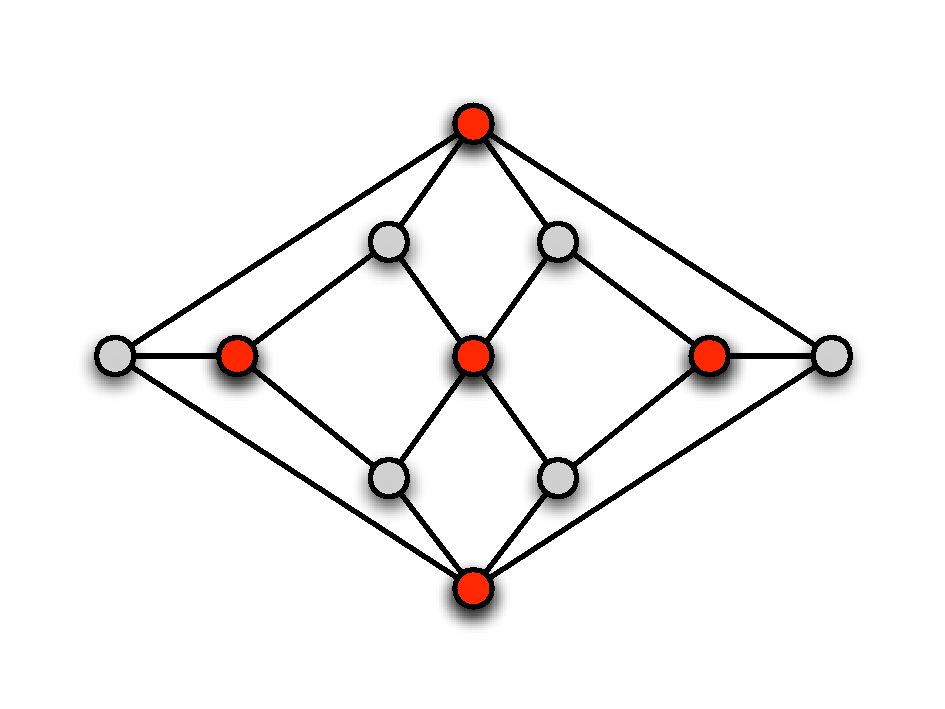
\includegraphics[width=10cm]{pic1.pdf}
    \end{center}
\caption{Herschelov graf, vektorska grafika.}
\label{pic1}
\end{figure}
Pa res lahko vključimo slike katerihkoli formatov? Žal ne. Programski paket \LaTeX\ lahko uporabljamo v več dialektih. Ukaz {\tt latex} ne mara vključenih slik v formatu Portable Document Format {\tt .pdf}, ukaz {\tt pdflatex} pa ne prebavi slik v Encapsulated Postscript Formatu {\tt .eps}.
Strnjeno v Tabeli~\ref{tbl:1}.

\begin{table}
    \begin{center}
        \begin{tabular}{l|ccc}
            ukaz/format & {\tt .pdf} & {\tt .eps} & ostali formati \\ \hline
                        {\tt pdflatex} & da & ne & da \\
                        {\tt latex}   & ne & da  & da
        \end{tabular}
    \end{center}
\caption{}
\label{tbl:1}
\end{table}

Nasvet? Odločite se za uporabo ukaza {\tt pdflatex}. Vaš izdelek bo brez vmesnih stopenj na voljo v {.pdf} formatu in ga lahko odnesete v vsako tiskarno. Če morate na vsak način vključiti sliko, ki jo imate v {\tt .eps} formatu, jo vnaprej pretvorite v alternativni format, denimo {\tt .pdf}.

Včasih se da v okolju za uporabo programskega paketa \LaTeX\ nastaviti na kakšen način bomo prebavljali vhodne dokumente. Spustni meni na Sliki~\ref{pic2} odkriva uporabo \LaTeX{}a v njegovi pdf inkarnaciji --- {\tt pdflatex}.
\begin{figure}
\begin{center}
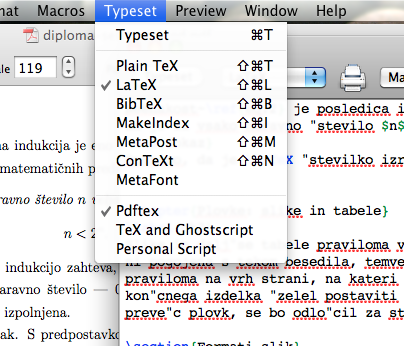
\includegraphics[width=10cm]{pic2.png}
\end{center}
\caption{Kateri dialekt uporabljati?}
\label{pic2}
\end{figure}

Vključena Slika~\ref{pic2} je seveda bitna.

Kaj pa stran iz študentskega referata?\label{pp}
Tudi njo lahko vključimo v dokument. Toda ne kot plovko.


%\chapter{}

\chapter{Kaj pa literatura?}
\label{ch3}
Kot smo omenili že v uvodu, je pravi način za citiranje literature uporaba \BibTeX{}a~\cite{bib}.
Programski paket \LaTeX je prvotno predstavljen v priročniku~\cite{lat} in je v resnici nadgradnja sistema \TeX\ avtorja Donalda Knutha, znanega po denimo, če izpustim njegovo umetnost programiranja, Knuth-Bendixovem algoritmu~\cite{dk1}.

Vsem raziskovalcem s področja računalništva pa svetujem v branje mnenje L.\ Fortnowa~\cite{lf}~\cite{trifonova}.

\chapter{Sklepne ugotovitve}
Izbira \LaTeX\ ali ne \LaTeX\ je seveda prepuščena vam samim. Res je, da so prvi koraki v \LaTeX{}u težavni. Ta dokument naj vam služi kot začetna opora pri hoji.

\printbibliography

\end{document}
